\section*{Multi-level ($\geq 2$) page table: an example}
\begin{tabular}{lllll}
  \hline
  VA bit & VA page size & Offset bit & PTE size & PDE size \\
  \hline
  30           & 512 byte     & $log_2 512 = 9$ & 4 byte & 4 byte \\
  \hline
\end{tabular}

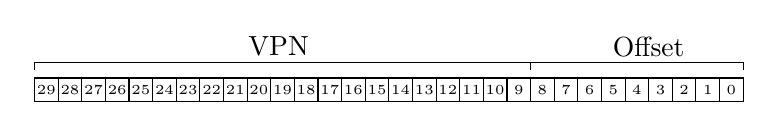
\begin{tikzpicture}
  % VPN
  \node at (3.1,0.7) (vpn){VPN};
  \draw (0, 0.4) -- (0,0.5);
  \draw (6.3, 0.4) -- (6.3,0.5);
  \draw (0, 0.5) -- (6.3,0.5);

  % Offset
  \node at (7.8,0.7) (off){Offset};
  \draw (6.3, 0.4) -- (6.3,0.5);
  \draw (9, 0.4) -- (9,0.5);
  \draw (6.3, 0.5) -- (9,0.5);

  \foreach \x [count=\xi from 0, evaluate=\xi as \num using int(29-\xi)] in
  {0,0.3,0.6,...,9}
  {
    \draw (\x, 0) rectangle (\x+0.3, 0.3);
    \node[font=\tiny] at (\x+0.15, 0.15) {\num};
  }
\end{tikzpicture}
\begin{itemize}
\item When chopping page table into pages, page table pages (PTP) usually have same \textbf{size} as virtual addr page: $S_{\text{VAP}} = S_{\text{PTP}} = 512$ bytes
\item Thus, each PTP will have $N_{\text{PTE}} = \frac{S_{\text{PTP}}}{S_{\text{PTE}}} = \frac{512}{4} = 128$ PTEs
\item To find each PTE, \texttt{PTIndex} need bits of $\log_2 N_{\text{PTE}} = \log_2 128 = 7$
\item The left 14 bits (30 - offset - \texttt{PTIndex}) used for Page Directory Index
\end{itemize}
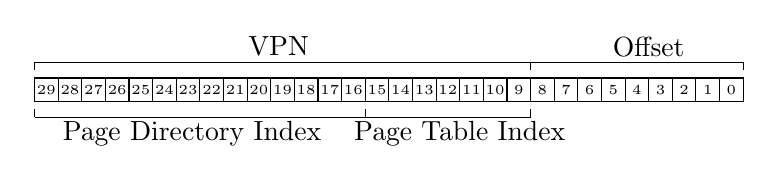
\begin{tikzpicture}
  % VPN
  \node at (3.1,0.7) (vpn){VPN};
  \draw (0, 0.4) -- (0,0.5);
  \draw (6.3, 0.4) -- (6.3,0.5);
  \draw (0, 0.5) -- (6.3,0.5);

  % Offset
  \node at (7.8,0.7) (off){Offset};
  \draw (6.3, 0.4) -- (6.3,0.5);
  \draw (9, 0.4) -- (9,0.5);
  \draw (6.3, 0.5) -- (9,0.5);

  \foreach \x [count=\xi from 0, evaluate=\xi as \num using int(29-\xi)] in
  {0,0.3,0.6,...,9}
  {
    \draw (\x, 0) rectangle (\x+0.3, 0.3);
    \node[font=\tiny] at (\x+0.15, 0.15) {\num};
  }

  % PDIndex
  \draw (0, -0.1) -- (0,-0.2);
  \draw (4.2, -0.1) -- (4.2,-0.2);
  \draw (0, -0.2) -- (4.2,-0.2);
  \node at (2,-0.4) (pdindex){Page Directory Index};

  % PTIndex
  \draw (4.2, -0.1) -- (4.2,-0.2);
  \draw (6.3, -0.1) -- (6.3,-0.2);
  \draw (4.2, -0.2) -- (6.3,-0.2);
  \node at (5.4,-0.4) (ptindex){Page Table Index};
\end{tikzpicture}
\begin{itemize}
\item this results in a \textbf{HUGE} PD itself: $2^{14}$ PEDs and requires 128 pages
\end{itemize}
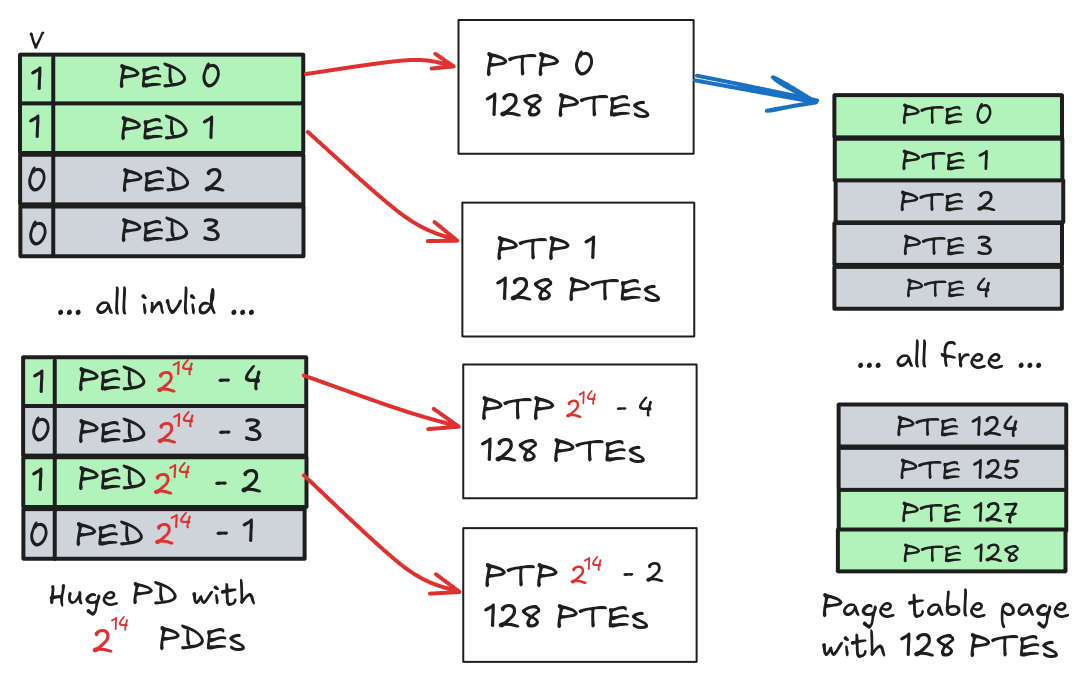
\includegraphics[width=\linewidth]{imgs/huge_2level_pt}
\begin{itemize}
\item Splitting PD into 2 levels and each level has same bit width: 7
\item TLB miss causes additional memory accesses
\end{itemize}
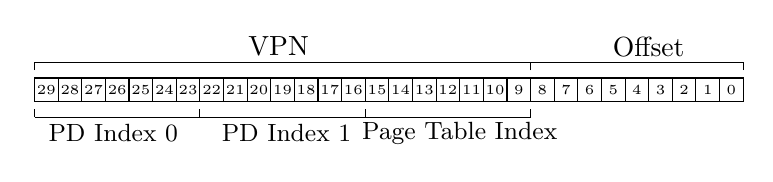
\begin{tikzpicture}
  % VPN
  \node at (3.1,0.7) (vpn){VPN};
  \draw (0, 0.4) -- (0,0.5);
  \draw (6.3, 0.4) -- (6.3,0.5);
  \draw (0, 0.5) -- (6.3,0.5);

  % Offset
  \node at (7.8,0.7) (off){Offset};
  \draw (6.3, 0.4) -- (6.3,0.5);
  \draw (9, 0.4) -- (9,0.5);
  \draw (6.3, 0.5) -- (9,0.5);

  \foreach \x [count=\xi from 0, evaluate=\xi as \num using int(29-\xi)] in
  {0,0.3,0.6,...,9}
  {
    \draw (\x, 0) rectangle (\x+0.3, 0.3);
    \node[font=\tiny] at (\x+0.15, 0.15) {\num};
  }

  % PDIndex 0
  \draw (0,   -0.1) -- (0,  -0.2);
  \draw (2.1, -0.1) -- (2.1,-0.2);
  \draw (0,   -0.2) -- (2.1,-0.2);
  \node at (1,-0.4) (pdindex0){\small PD Index 0};

  % PDIndex 1
  \draw (4.2, -0.1) -- (4.2,-0.2);
  \draw (2.1, -0.2) -- (4.2,-0.2);
  \node at (3.2,-0.4) (pdindex1){\small PD Index 1};

  % PTIndex 0
  \draw (4.2, -0.1) -- (4.2,-0.2);
  \draw (6.3, -0.1) -- (6.3,-0.2);
  \draw (4.2, -0.2) -- (6.3,-0.2);
  \node at (5.4,-0.4) (ptindex){\small Page Table Index};
\end{tikzpicture}

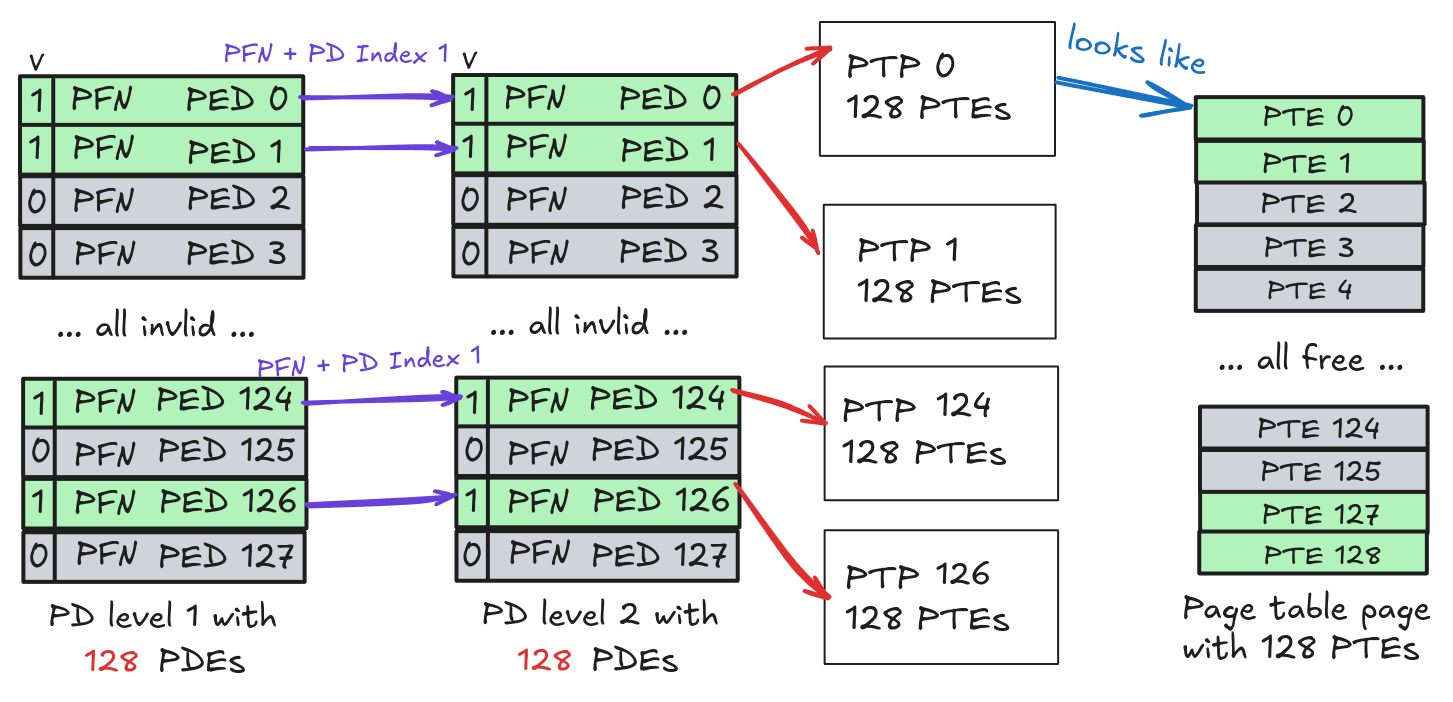
\includegraphics[width=\linewidth]{imgs/smaller_3level_pt}

\begin{itemize}
\item the bigger the page table, the faster a TLB miss can be serviced
\item memory-constrained (old) system, smaller page tables preferred
\end{itemize}
